\documentclass{article}

\usepackage{graphicx}

\title{Data Visualization 1}
\author{Divij Singh}
\date{19/02/18}

\begin{document}

	\maketitle
	
	The data represented below is a comparison of the amount each video game I own on the Steam gaming platform costs, versus the amount of time I have spent playing it. The data is taken using SteamDB (an online tool for information about your account), and cleaned using Microsoft Excel. The graph was made using Chartblocks This dataset comprises of 370 games.\\
	\\
	I decided to present it as a scatter plot, as it allows you to compare games which have low cost but high playtime, and high playtime but low cost.\\
	\\
	One surprising observation I made was that my two most played games are both free games, whereas I own a number of games worth over Rs. 1000 which I haven't played at all.\\
	\\
	A question to be considered is why the playtime of the free games is so high, versus the low playtime of more expensive games, when one would expect the opposite.\\
	\\
	
	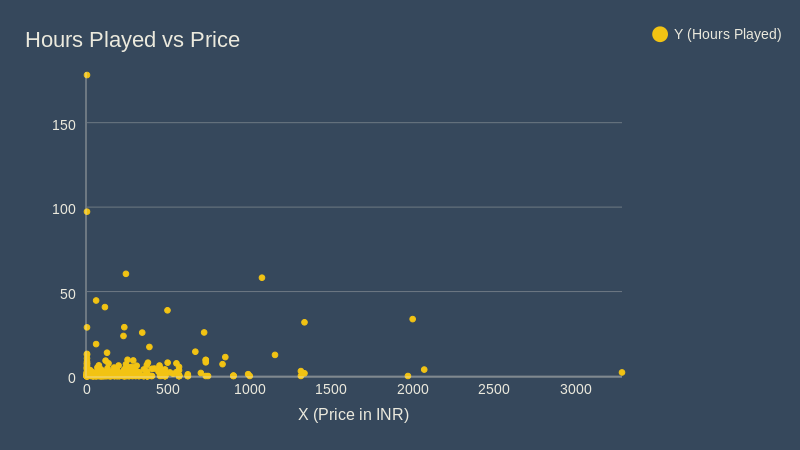
\includegraphics[width=\textwidth]{scatter_plot}
	
	
\end{document}